\hsection{Violation:~{T}he Use of Multivalued Attributes}%
\FloatBarrier%
%
\begin{figure}%
\centering%
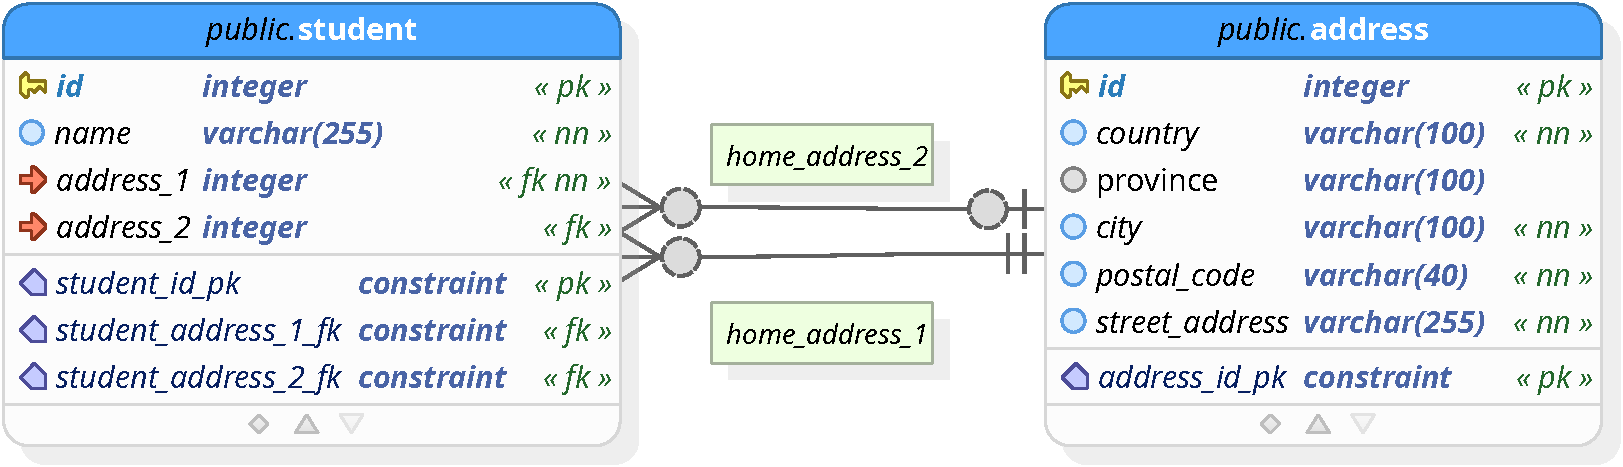
\includegraphics[width=0.6\linewidth]{\currentDir/anomalyMultivalued}%
\caption{A violation of the \pgls{1NF}:~{T}he \sqlil{student} table has two fields referencing addresses to simulate a multivalued attribute.}%
\label{fig:anomalyMultivalued}%
\end{figure}%
%
\gitExec{\databasesCodeRepo}{.}{_scripts_/postgres.sh normalization/1nf/anomaly_multivalued/generated_sql 01_anomalies_database_2001.sql}%
\gitExec{\databasesCodeRepo}{.}{_scripts_/postgres.sh normalization/1nf/anomaly_multivalued/generated_sql 03_public_address_table_5071.sql anomalies}%
%
\gitSQL{\databasesCodeRepo}{normalization/1nf/anomaly_multivalued/generated_sql/04_public_student_table_5079.sql}{1nf:anomaly_multivalued:04_public_student_table_5079}{The generated \sql\ code for creating the \sqlil{student} table with two columns for addresses based on \cref{fig:anomalyMultivalued}, which violates the \pgls{1NF}.}%
\gitExec{\databasesCodeRepo}{.}{_scripts_/postgres.sh normalization/1nf/anomaly_multivalued/generated_sql 04_public_student_table_5079.sql anomalies}%
\gitExec{\databasesCodeRepo}{.}{_scripts_/postgres.sh normalization/1nf/anomaly_multivalued/generated_sql 05_public_student_student_address_1_fk_constraint_5085.sql anomalies}%
\gitExec{\databasesCodeRepo}{.}{_scripts_/postgres.sh normalization/1nf/anomaly_multivalued/generated_sql 06_public_student_student_address_2_fk_constraint_5086.sql anomalies}%
%
\gitSQL{\databasesCodeRepo}{normalization/1nf/anomaly_multivalued/insert.sql}{normalization:1nf:anomaly_multivalued:insert}{%
Inserting some data into the tables~\sqlil{student} and~\sqlil{address} in violation of the \pgls{1NF} based on \cref{fig:anomalyMultivalued}.}%
\gitExec{\databasesCodeRepo}{.}{_scripts_/postgres.sh normalization/1nf/anomaly_multivalued insert.sql anomalies}%
%
\gitSQLAndOutput{\databasesCodeRepo}{normalization/1nf/anomaly_multivalued}{select.sql}{anomalies}{}{}{postgres.sh}{normalization:1nf:anomaly_multivalued:select}{%
Trying to find all the students with at least one address in China, which is harder than necessary, because table \sqlil{student} violates the \pgls{1NF}.}%
%
\gitExec{\databasesCodeRepo}{.}{_scripts_/postgres.sh normalization/1nf/anomaly_multivalued cleanup.sql}%
%
Let us continue our example from the previous section.
There, we developed a two-table structure for storing addresses of students.
Each student had exactly one address.
But maybe in reality, students can have more than one address.
Let's say their current address, maybe in the university dormitory in a flat rented nearby, and their old home address, i.e., the flat of their parents.
In the model from the previous section, this cannot be implemented.
In \cref{fig:anomalyMultivalued}, the \db\ developer had a very simple idea:
Let's just have two columns for the addresses -- \sqlil{address_1} and \sqlil{address_2} -- in the table~\sqlil{student}.
By doing so, they have violated the \pgls{1NF}.
\FloatBarrier%
\endhsection%
%
